\subsubsection{Presentation}
\label{ch:deepar}
We'll start the presentation of this algorithm by quoting \href{https://docs.aws.amazon.com/sagemaker/latest/dg/deepar.html}{AWS on DeepAR}  \cite{awsdeepar}:
\begin{displayquote}
"The Amazon SageMaker DeepAR forecasting algorithm is a supervised learning algorithm for forecasting scalar (one-dimensional) time series using recurrent neural networks (RNN). Classical forecasting methods, such as autoregressive integrated moving average (ARIMA) or exponential smoothing (ETS), fit a single model to each individual time series. They then use that model to extrapolate the time series into the future."
\end{displayquote}

\begin{figure}[h!]
    \centering
    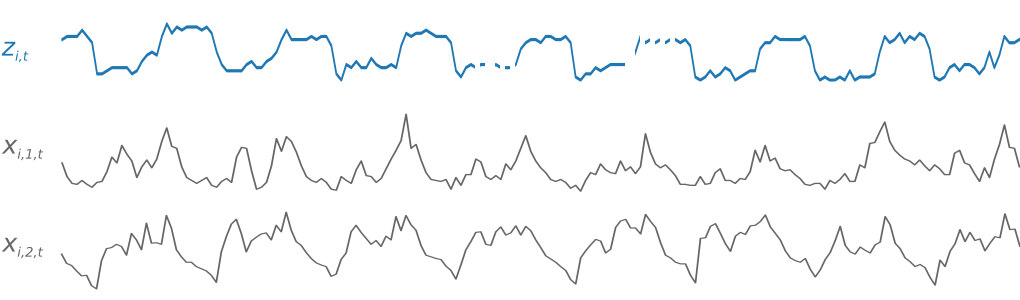
\includegraphics[width=1\textwidth]{images/deepar-explanation.png}
    \caption{DeepAR learns to predict a target (in blue), possibly from dynamic features (in black)}
    \label{fig:deepar-explanation}
\end{figure}


\subsubsection{Use-cases}

The strength of this algorithm resides in the fact that it is able to learn simultaneously from different correlated time series (called \lstinline{targets}) and their associated \lstinline{dynamic features}, which are additionnal time series used as features during training. Please note that it can't be trained on streaming data.

To take a concrete example, let's say we wish to predict the requests hitting the BMW servers on a per-city basis. Our \lstinline{targets} would be the weekly profile of requests coming from each major city, and the associated \lstinline{dynamic features} could for instance be the weekly profile of oil prices and temperatures in those cities.

For the sake of clarity, below is an example of what data shape DeepAR expects. Each line corresponds to a \lstinline{target} time series,  and each \lstinline{dynamic_feat} to a list of its associated dynamic features.


\begin{lstlisting}
{"start": "2009-11-01 00:00:00", "target": [4.3, "NaN", 5.1, ...], "cat": [0, 1], "dynamic_feat": [[1.1, 1.2, 0.5,...]]}
{"start": "2012-01-30 00:00:00", "target": [1.0, -5.0, ...], "cat": [2, 3], "dynamic_feat": [[1.1, 2.05, ...]]}
{"start": "1999-01-30 00:00:00", "target": [2.0, 1.0], "cat": [1, 4], "dynamic_feat": [[1.3, 0.4]]}
\end{lstlisting}

As a further remark, one can point out that DeepAR supports unknown target values during training, which can be useful if we have an outage at some point cutting access to the data stream.

\subsubsection{Behavior on the BMW dataset}

We tried three different approaches with the DeepAR algorithm, all having a common agreement: train on all the dataset but the last week, and test on the last week. \\
It is useful to remark that one could have removed the part of the data being the christmas holidays, but we were curious about the ability of DeepAR to abstract these "outliers". We trained with the following parameters:

\begin{enumerate}
    \item \textbf{Training without dynamic features}
    \begin{enumerate}
        \item[] \textbf{Idea}:\\
        Training set on all data but the last week, performance evaluation on the last week, without any dynamic features.
        \item[] \textbf{Input shape}: \\
        \begin{lstlisting}
        {"start": "2019-11-01 00:00:00", "target": [4.3, "NaN", 5.1, ...]}
        \end{lstlisting}

        \item[] \textbf{Results}:\\
        \begin{figure}[h!]
            \centering
            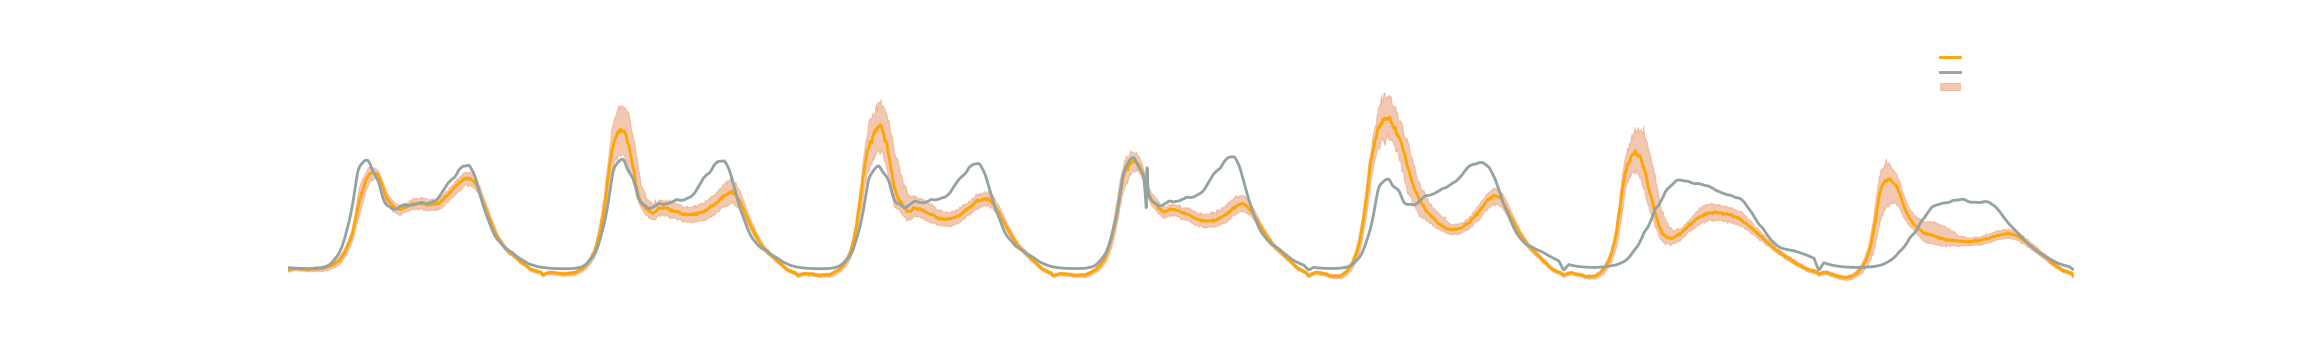
\includegraphics[width=1\textwidth]{images/deepar_no_dyn.png}
            \caption{DeepAR Prediction trained without dynamic features.}
            \description{}
            \label{fig:deepar_no_dyn}
        \end{figure}
        Remarkably, the algorithm performs quite well during the working days with a RMSE (Root Mean Square Error) of 95K. but is unable to learn the trends of weekends. This is quite interesting, since DeepAR is supposed under the hood to automatically encode additional temporal information such as the day of week. Maybe adding some hidden neurons would improve its ability to learn the weekend patterns.
        
    \end{enumerate}
    
    \item \textbf{1-Week forecasting training with holidays features}
    \begin{itemize}
        \item[] \textbf{Idea}:\\
        Training set on all data but the last week, performance evaluation on the last week, with holidays dynamic features. When a day is a holiday, its associated dynamic feature is a one, else 0. \\
        We train the model to predict a full week , with a week of context.
        \item[] \textbf{Input shape}:\\
        \begin{lstlisting}
        {"start": "2019-11-01 00:00:00", "target": [4.3, "NaN", 5.1, ...], "dynamic_feat": [[0, 0, 1,...]]}
        \end{lstlisting}
        \item[] \textbf{Results}:\\
        \textbf{RMSE (Root Mean Square Deviation) of 72K}
    \end{itemize}
    
    \item \textbf{1-Week forecasting training with holidays \& weekends features}
    \begin{itemize}
        \item[] \textbf{Idea}:\\
        Training set on all data but the last week, performance evaluation on the last week, with holidays \& weekends dynamic features. When a day is a holiday, its associated dynamic feature is a one, else 0. And similarly, when a day is a weekend, its associated feature is a one, else 0. We decided to add the weekends feature since in the first part we identified that DeepAR had trouble learning their pattern.\\
        We train the model to predict a full week , with a week of context.

        \item[] \textbf{Input shape}:\\
        \begin{lstlisting}
        {"start": "2019-11-01 00:00:00", "target": [4.3, "NaN", 5.1, ...], "dynamic_feat": [[0, 0, 1,...],[1, 1, 0, 0, ...]}
        \end{lstlisting}

        \item[] \textbf{Results}:\\
        \textbf{RMSE (Root Mean Square Deviation) of 122K }
        Adding the weekends dynamic features deeply worsened the model performance, and we think this is because it might conflict with what DeepAR does already perform under the hood. This shows that adding extra dynamic features do not necessary improve this model.
    \end{itemize}
    

    \item \textbf{3H forecasting training with holidays \& weekends features}
    \begin{itemize}
        \item[] \textbf{Idea}:\\
        Training set on all data but the last week, performance evaluation on the last week, with holidays \& weekends dynamic features. When a day is a holiday, its associated dynamic feature is a one, else 0. And similarly, when a day is a weekend, its associated feature is a one, else 0.  \\
        The main idea behind this is to have a higher hourly granularity during the forecast, this being useful for instance during predictive auto-scaling.
        
        \item[] \textbf{Input shape}:\\
        \begin{lstlisting}
        {"start": "2019-11-01 00:00:00", "target": [4.3, "NaN", 5.1, ...], "dynamic_feat": [[0, 0, 1,...],[1, 1, 0, 0, ...]]}
        \end{lstlisting}
        \item[] \textbf{Results}:\\
        \textbf{RMSE (Root Mean Square Deviation) of 132K}
        For some reason, this tuning of the algorithm did  perform poorly. One of our guess is that the data aggregated in 5-min buckets is too broad, and that we should rather aggregate it in 1-min buckets. Also, it is possible that we are working with too little data as well.
    \end{itemize}
\end{enumerate}


\subsubsection{Discussion and recommendations}

\begin{itemize}
    \item[] As mentionned in AWS description, DeepAR outperforms traditional time series forecasting algorithms when the dataset comprises thousands of correlated time series. We tested it on a single time series coupled with only two dynamic features, but it already had promising results (see \ref{fig:deepar_no_dyn}), improving continuously with the number of dynamic features.
    
    \item[] However, even though DeepAR is supposed to generate additional time features such as day of week, it did not perform well on weekends, and we had to input these features dynamically. This leads us to believe that there is a bit of tweaking to do in order to obtain a foolproof model.
    
    \item[] Due to the lack of geolocalized data, we tested this algorithm on a simple task, whereas it is designed to work on a lot more complex task. Thus, we highly recommend that you try it \textbf{when additional, geolocalized data will be available, such as traffic per world area. In this case, DeepAR could outperform traditional models and give BMW valuable insight}.
\end{itemize} 